\documentclass[11pt, letterpaper]{article}

% Fonts and Encoding
\usepackage[utf8]{inputenc}
\usepackage[T1]{fontenc}
\usepackage{lmodern} % High-quality Latin Modern vector font

% Math and Symbols
\usepackage{amsmath, amssymb, amsthm, amsfonts, mathrsfs, mathtools}

% Layout and Geometry
\usepackage{geometry}
\geometry{letterpaper, margin=1in}
\setlength{\parindent}{0pt}
\setlength{\parskip}{0.6em}

% Formatting and Graphics
\usepackage{graphicx, xcolor, enumitem, booktabs, array, tabularx}

% TikZ for Illustrations
\usepackage{tikz}
\usetikzlibrary{arrows.meta, positioning, shapes.geometric, calc, backgrounds, matrix}

% Clickable Links and TOC
\usepackage{hyperref}
\hypersetup{
    colorlinks=true,
    linkcolor=blue,
    filecolor=magenta,      
    urlcolor=cyan,
    pdftitle={Constrained Optimization},
}

% Theorem Environments
\newtheorem{theorem}{Theorem}[section]
\newtheorem{lemma}[theorem]{Lemma}
\newtheorem{proposition}[theorem]{Proposition}
\newtheorem{corollary}[theorem]{Corollary}
\theoremstyle{definition}
\newtheorem{definition}{Definition}[section]
\newtheorem{axiom}{Axiom}[section]
\newtheorem{example}{Example}[section]
\theoremstyle{remark}
\newtheorem{remark}{Remark}[section]

% Custom Commands (Enforced standard notation)
\newcommand{\R}{\mathbb{R}}
\newcommand{\N}{\mathbb{N}}
\newcommand{\Z}{\mathbb{Z}}
\newcommand{\Q}{\mathbb{Q}}
\newcommand{\E}{\mathbb{E}}
\newcommand{\Prob}{\mathbb{P}}
\newcommand{\F}{\mathcal{F}}

\begin{document}

\title{\textbf{Mastery Guide: Constrained Optimization}}
\author{Tashfeen Omran}
\date{}
\maketitle

\tableofcontents
\newpage

\section{Part 1: Comprehensive Introduction, Context, and Prerequisites}

\subsection{Core Concepts}
Constrained Optimization, in the context of linear algebra, deals with finding the maximum or minimum values of a quadratic form $Q(\mathbf{x}) = \mathbf{x}^T A \mathbf{x}$ subject to a specific geometric boundary, most commonly the unit sphere defined by $\|\mathbf{x}\| = 1$ (or equivalently, $\mathbf{x}^T\mathbf{x} = 1$). 

When a quadratic form has no cross-product terms (i.e., its matrix $A$ is diagonal), finding the maximum and minimum on the unit sphere is trivial: they are simply the largest and smallest diagonal entries. However, when cross-product terms exist, the matrix $A$ is symmetric but not diagonal. The core concept of this section is that by orthogonally diagonalizing $A$, we can rotate our coordinate system to align with the principal axes of the quadratic form, thereby eliminating the cross-product terms and revealing the true maximum and minimum values as the eigenvalues of $A$.

\subsection{Intuition and Derivation}
Why do eigenvalues represent the maximum and minimum values? Consider the orthogonal diagonalization of a symmetric matrix $A = P D P^T$, where $P$ is an orthogonal matrix of eigenvectors and $D$ is a diagonal matrix of eigenvalues. 
If we apply the change of variable $\mathbf{x} = P\mathbf{y}$, the quadratic form becomes:
\[ Q(\mathbf{x}) = \mathbf{x}^T A \mathbf{x} = (P\mathbf{y})^T A (P\mathbf{y}) = \mathbf{y}^T (P^T A P) \mathbf{y} = \mathbf{y}^T D \mathbf{y} \]
Because $P$ is an orthogonal matrix, it preserves length. Thus, the constraint $\|\mathbf{x}\| = 1$ is perfectly equivalent to $\|\mathbf{y}\| = 1$. The transformed quadratic form is simply $\lambda_1 y_1^2 + \lambda_2 y_2^2 + \dots + \lambda_n y_n^2$. If we order the eigenvalues such that $\lambda_1 \ge \lambda_2 \ge \dots \ge \lambda_n$, it is algebraically clear that the maximum value on the unit sphere is $\lambda_1$ (achieved when $y_1 = 1$ and all other $y_i = 0$), and the minimum is $\lambda_n$.

\subsection{Historical Context and Motivation}
The mathematical foundation for optimizing quadratic forms was laid in the 19th century by mathematicians such as Augustin-Louis Cauchy and Karl Weierstrass. The primary motivation came from classical mechanics—specifically, the study of rigid body dynamics and the search for "principal axes of inertia." Physicists needed to find coordinate systems where the rotational inertia matrix became diagonal, simplifying the equations of motion. This purely physical problem birthed the spectral theorem for symmetric matrices, which now serves as the engine for modern optimization, statistics, and machine learning.

\subsection{Key Formulas and Theorems}
\begin{itemize}
    \item \textbf{Quadratic Form:} $Q(\mathbf{x}) = \mathbf{x}^T A \mathbf{x}$
    \item \textbf{Unit Vector Constraint:} $\mathbf{x}^T\mathbf{x} = 1$ (or $x_1^2 + x_2^2 + \dots + x_n^2 = 1$)
    \item \textbf{Theorem 6 (Absolute Extrema):} Let $A$ be a symmetric matrix. The maximum value of $\mathbf{x}^T A \mathbf{x}$ subject to $\mathbf{x}^T\mathbf{x} = 1$ is the greatest eigenvalue $\lambda_1$. This maximum is attained at the corresponding unit eigenvector $\mathbf{u}_1$. The minimum is the least eigenvalue $\lambda_n$, attained at $\mathbf{u}_n$.
    \item \textbf{Theorem 7 (Orthogonal Constraints):} The maximum value of $\mathbf{x}^T A \mathbf{x}$ subject to $\mathbf{x}^T\mathbf{x} = 1$ \textit{and} $\mathbf{x}^T\mathbf{u}_1 = 0$ is the second greatest eigenvalue $\lambda_2$, attained at $\mathbf{u}_2$.
\end{itemize}

\subsection{Prerequisites}
To succeed in this topic, you must be fluent in:
1. \textbf{Eigenvalues and Eigenvectors:} Solving $\det(A - \lambda I) = 0$ and finding the null space of $A - \lambda I$.
2. \textbf{Symmetric Matrices:} Understanding that symmetric matrices always yield real eigenvalues and orthogonal eigenvectors.
3. \textbf{Orthogonal Matrices:} Knowing that $P^T = P^{-1}$ and that multiplying by $P$ preserves vector length.
4. \textbf{Quadratic Forms:} Translating a polynomial like $ax_1^2 + bx_2^2 + cx_1x_2$ into a symmetric matrix $A$.

\newpage

\section{Part 2: Detailed Homework Solutions}

\subsection{Exercises 1--2: Change of Variable}

\textbf{Problem 1:} Find the change of variable $\mathbf{x} = P\mathbf{y}$ that transforms the quadratic form $5x_1^2 + 4x_2^2 + 3x_3^2 + 4x_1x_2 + 4x_2x_3$ into $7y_1^2 + 4y_2^2 + y_3^2$.

\textbf{Solution:}
First, we extract the symmetric matrix $A$ from the original quadratic form $Q(\mathbf{x})$. The diagonal entries are the coefficients of the squared terms, and the off-diagonal entries are half the coefficients of the cross-product terms.
\[ A = \begin{bmatrix} 5 & 2 & 0 \\ 2 & 4 & 2 \\ 0 & 2 & 3 \end{bmatrix} \]
The target quadratic form tells us that the eigenvalues of $A$ are $\lambda_1 = 7$, $\lambda_2 = 4$, and $\lambda_3 = 1$. We must find the corresponding orthonormal eigenvectors to construct $P$.

\textit{Step 1: Eigenvector for $\lambda_1 = 7$}
\[ A - 7I = \begin{bmatrix} -2 & 2 & 0 \\ 2 & -3 & 2 \\ 0 & 2 & -4 \end{bmatrix} \]
Solving $(A - 7I)\mathbf{x} = \mathbf{0}$: The first row gives $-2x_1 + 2x_2 = 0 \implies x_1 = x_2$. The third row gives $2x_2 - 4x_3 = 0 \implies x_2 = 2x_3$. Let $x_3 = 1$, then $x_2 = 2$ and $x_1 = 2$. The vector is $(2, 2, 1)^T$. Normalizing it (length is $\sqrt{4+4+1} = 3$), we get $\mathbf{u}_1 = \begin{bmatrix} 2/3 \\ 2/3 \\ 1/3 \end{bmatrix}$.

\textit{Step 2: Eigenvector for $\lambda_2 = 4$}
\[ A - 4I = \begin{bmatrix} 1 & 2 & 0 \\ 2 & 0 & 2 \\ 0 & 2 & -1 \end{bmatrix} \]
Row 1 gives $x_1 + 2x_2 = 0 \implies x_1 = -2x_2$. Row 3 gives $2x_2 - x_3 = 0 \implies x_3 = 2x_2$. Let $x_2 = 1$, then $x_1 = -2$ and $x_3 = 2$. The vector is $(-2, 1, 2)^T$. Normalizing yields $\mathbf{u}_2 = \begin{bmatrix} -2/3 \\ 1/3 \\ 2/3 \end{bmatrix}$.

\textit{Step 3: Eigenvector for $\lambda_3 = 1$}
\[ A - I = \begin{bmatrix} 4 & 2 & 0 \\ 2 & 3 & 2 \\ 0 & 2 & 2 \end{bmatrix} \]
Row 1 gives $4x_1 + 2x_2 = 0 \implies x_2 = -2x_1$. Row 3 gives $2x_2 + 2x_3 = 0 \implies x_3 = -x_2 = 2x_1$. Let $x_1 = 1$, then $x_2 = -2$ and $x_3 = 2$. The vector is $(1, -2, 2)^T$. Normalizing yields $\mathbf{u}_3 = \begin{bmatrix} 1/3 \\ -2/3 \\ 2/3 \end{bmatrix}$.

\textit{Final Answer:} The change of variable matrix is $P = \begin{bmatrix} \mathbf{u}_1 & \mathbf{u}_2 & \mathbf{u}_3 \end{bmatrix}$.
\[ \mathbf{x} = \begin{bmatrix} 2/3 & -2/3 & 1/3 \\ 2/3 & 1/3 & -2/3 \\ 1/3 & 2/3 & 2/3 \end{bmatrix} \mathbf{y} \]

\vspace{1em}
\textbf{Problem 2:} Find the change of variable $\mathbf{x} = P\mathbf{y}$ that transforms $5x_1^2 + 5x_2^2 + 3x_3^2 + 10x_1x_2 + 4x_1x_3 + 4x_2x_3$ into $11y_1^2 + 2y_2^2$.

\textbf{Solution:}
The symmetric matrix $A$ is:
\[ A = \begin{bmatrix} 5 & 5 & 2 \\ 5 & 5 & 2 \\ 2 & 2 & 3 \end{bmatrix} \]
The target form $11y_1^2 + 2y_2^2 + 0y_3^2$ indicates eigenvalues $\lambda_1 = 11$, $\lambda_2 = 2$, and $\lambda_3 = 0$.

\textit{Step 1: Eigenvector for $\lambda_1 = 11$}
\[ A - 11I = \begin{bmatrix} -6 & 5 & 2 \\ 5 & -6 & 2 \\ 2 & 2 & -8 \end{bmatrix} \]
Subtracting row 2 from row 1 gives $-11x_1 + 11x_2 = 0 \implies x_1 = x_2$. Substituting into row 3: $2(x_1) + 2(x_1) - 8x_3 = 0 \implies 4x_1 = 8x_3 \implies x_1 = 2x_3$. Let $x_3 = 1$, then $x_1 = 2, x_2 = 2$. Normalized: $\mathbf{u}_1 = \begin{bmatrix} 2/3 \\ 2/3 \\ 1/3 \end{bmatrix}$.

\textit{Step 2: Eigenvector for $\lambda_2 = 2$}
\[ A - 2I = \begin{bmatrix} 3 & 5 & 2 \\ 5 & 3 & 2 \\ 2 & 2 & 1 \end{bmatrix} \]
Subtracting row 2 from row 1 gives $-2x_1 + 2x_2 = 0 \implies x_1 = x_2$. Substituting into row 3: $2x_1 + 2x_1 + x_3 = 0 \implies x_3 = -4x_1$. Let $x_1 = 1$, then $x_2 = 1, x_3 = -4$. Length is $\sqrt{1+1+16} = \sqrt{18} = 3\sqrt{2}$. Normalized: $\mathbf{u}_2 = \begin{bmatrix} 1/(3\sqrt{2}) \\ 1/(3\sqrt{2}) \\ -4/(3\sqrt{2}) \end{bmatrix}$.

\textit{Step 3: Eigenvector for $\lambda_3 = 0$}
\[ A - 0I = \begin{bmatrix} 5 & 5 & 2 \\ 5 & 5 & 2 \\ 2 & 2 & 3 \end{bmatrix} \]
Row 1 and Row 3: $5x_1 + 5x_2 + 2x_3 = 0$ and $2x_1 + 2x_2 + 3x_3 = 0$. Multiplying row 3 by 2 and subtracting from 3 times row 1 eliminates $x_1, x_2$, forcing $x_3 = 0$. Then $5x_1 + 5x_2 = 0 \implies x_1 = -x_2$. Let $x_1 = 1$, then $x_2 = -1, x_3 = 0$. Normalized: $\mathbf{u}_3 = \begin{bmatrix} 1/\sqrt{2} \\ -1/\sqrt{2} \\ 0 \end{bmatrix}$.

\textit{Final Answer:} 
\[ \mathbf{x} = \begin{bmatrix} 2/3 & \frac{1}{3\sqrt{2}} & \frac{1}{\sqrt{2}} \\ 2/3 & \frac{1}{3\sqrt{2}} & -\frac{1}{\sqrt{2}} \\ 1/3 & -\frac{4}{3\sqrt{2}} & 0 \end{bmatrix} \mathbf{y} \]

\subsection{Exercises 3--6: Maximums and Orthogonal Constraints}

\textbf{Problem 3:} For $Q(\mathbf{x}) = 5x_1^2 + 4x_2^2 + 3x_3^2 + 4x_1x_2 + 4x_2x_3$, find (a) max of $Q(\mathbf{x})$ subject to $\mathbf{x}^T\mathbf{x}=1$, (b) unit vector $\mathbf{u}$ where max is attained, (c) max of $Q(\mathbf{x})$ subject to $\mathbf{x}^T\mathbf{x}=1$ and $\mathbf{x}^T\mathbf{u}=0$.

\textbf{Solution:}
From Exercise 1, the eigenvalues are $7, 4, 1$.
(a) By Theorem 6, the maximum value is the greatest eigenvalue: $\lambda_1 = 7$.
(b) The maximum is attained at the corresponding unit eigenvector: $\mathbf{u} = \begin{bmatrix} 2/3 \\ 2/3 \\ 1/3 \end{bmatrix}$.
(c) By Theorem 7, the maximum subject to the orthogonal constraint $\mathbf{x}^T\mathbf{u}=0$ is the second greatest eigenvalue: $\lambda_2 = 4$.

\vspace{1em}
\textbf{Problem 4:} For $Q(\mathbf{x}) = 5x_1^2 + 5x_2^2 + 3x_3^2 + 10x_1x_2 + 4x_1x_3 + 4x_2x_3$.

\textbf{Solution:}
From Exercise 2, the eigenvalues are $11, 2, 0$.
(a) Maximum value is $\lambda_1 = 11$.
(b) Attained at $\mathbf{u} = \begin{bmatrix} 2/3 \\ 2/3 \\ 1/3 \end{bmatrix}$.
(c) Maximum subject to $\mathbf{x}^T\mathbf{u}=0$ is $\lambda_2 = 2$.

\vspace{1em}
\textbf{Problem 5:} For $Q(\mathbf{x}) = x_1^2 + x_2^2 - 12x_1x_2$.

\textbf{Solution:}
The matrix is $A = \begin{bmatrix} 1 & -6 \\ -6 & 1 \end{bmatrix}$.
Characteristic equation: $(1-\lambda)^2 - 36 = 0 \implies 1-\lambda = \pm 6 \implies \lambda = 7, -5$.
(a) Maximum value is $\lambda_1 = 7$.
(b) Find eigenvector for $\lambda = 7$: $A - 7I = \begin{bmatrix} -6 & -6 \\ -6 & -6 \end{bmatrix}$. Thus $x_1 = -x_2$. Normalized: $\mathbf{u} = \begin{bmatrix} 1/\sqrt{2} \\ -1/\sqrt{2} \end{bmatrix}$.
(c) Maximum subject to $\mathbf{x}^T\mathbf{u}=0$ is the second eigenvalue: $\lambda_2 = -5$.

\vspace{1em}
\textbf{Problem 6:} For $Q(\mathbf{x}) = 4x_1^2 + 7x_2^2 + 4x_1x_2$.

\textbf{Solution:}
The matrix is $A = \begin{bmatrix} 4 & 2 \\ 2 & 7 \end{bmatrix}$.
Characteristic equation: $(4-\lambda)(7-\lambda) - 4 = \lambda^2 - 11\lambda + 24 = (\lambda-8)(\lambda-3) = 0$. Eigenvalues are $8, 3$.
(a) Maximum value is $\lambda_1 = 8$.
(b) Find eigenvector for $\lambda = 8$: $A - 8I = \begin{bmatrix} -4 & 2 \\ 2 & -1 \end{bmatrix}$. Thus $2x_1 = x_2$. Normalized: $\mathbf{u} = \begin{bmatrix} 1/\sqrt{5} \\ 2/\sqrt{5} \end{bmatrix}$.
(c) Maximum subject to $\mathbf{x}^T\mathbf{u}=0$ is $\lambda_2 = 3$.

\subsection{Exercises 7--10: Finding the Maximum}

\textbf{Problem 7:} Let $Q(\mathbf{x}) = -3x_1^2 - 4x_2^2 + 4x_1x_2 - 4x_2x_3$. Find a unit vector $\mathbf{x}$ in $\R^3$ at which $Q(\mathbf{x})$ is maximized. [Hint: Eigenvalues are 1, -2, -6].

\textbf{Solution:}
The matrix is $A = \begin{bmatrix} -3 & 2 & 0 \\ 2 & -4 & -2 \\ 0 & -2 & 0 \end{bmatrix}$.
The maximum value is the largest eigenvalue, $\lambda = 1$. We find its eigenvector:
\[ A - I = \begin{bmatrix} -4 & 2 & 0 \\ 2 & -5 & -2 \\ 0 & -2 & -1 \end{bmatrix} \]
Row 1 gives $-4x_1 + 2x_2 = 0 \implies x_2 = 2x_1$. Row 3 gives $-2x_2 - x_3 = 0 \implies x_3 = -2x_2 = -4x_1$. Let $x_1 = 1$, then $x_2 = 2, x_3 = -4$. The length is $\sqrt{1^2 + 2^2 + (-4)^2} = \sqrt{21}$.
\textit{Final Answer:} $\mathbf{x} = \begin{bmatrix} 1/\sqrt{21} \\ 2/\sqrt{21} \\ -4/\sqrt{21} \end{bmatrix}$.

\vspace{1em}
\textbf{Problem 8:} Let $Q(\mathbf{x}) = 4x_1^2 + 7x_2^2 + 4x_3^2 - 4x_1x_2 + 8x_1x_3 + 4x_2x_3$. Find a unit vector $\mathbf{x}$ at which $Q(\mathbf{x})$ is maximized. [Hint: Eigenvalues are 8 and -1].

\textbf{Solution:}
The matrix is $A = \begin{bmatrix} 4 & -2 & 4 \\ -2 & 7 & 2 \\ 4 & 2 & 4 \end{bmatrix}$.
The maximum value is $\lambda = 8$. We find its eigenvector:
\[ A - 8I = \begin{bmatrix} -4 & -2 & 4 \\ -2 & -1 & 2 \\ 4 & 2 & -4 \end{bmatrix} \]
All rows are scalar multiples of $2x_1 + x_2 - 2x_3 = 0$. We need any unit vector satisfying this. Let $x_1 = 1, x_3 = 1$, then $x_2 = 0$. The vector is $(1, 0, 1)^T$. Normalizing gives length $\sqrt{2}$.
\textit{Final Answer:} $\mathbf{x} = \begin{bmatrix} 1/\sqrt{2} \\ 0 \\ 1/\sqrt{2} \end{bmatrix}$.

\vspace{1em}
\textbf{Problem 9:} Find the maximum value of $Q(\mathbf{x}) = 8x_1^2 + 6x_2^2 - 2x_1x_2$ subject to $x_1^2 + x_2^2 = 1$.

\textbf{Solution:}
The matrix is $A = \begin{bmatrix} 8 & -1 \\ -1 & 6 \end{bmatrix}$.
Characteristic equation: $(8-\lambda)(6-\lambda) - 1 = \lambda^2 - 14\lambda + 47 = 0$.
Using the quadratic formula: $\lambda = \frac{14 \pm \sqrt{196 - 188}}{2} = \frac{14 \pm \sqrt{8}}{2} = 7 \pm \sqrt{2}$.
The maximum value is the largest eigenvalue.
\textit{Final Answer:} $7 + \sqrt{2}$.

\vspace{1em}
\textbf{Problem 10:} Find the maximum value of $Q(\mathbf{x}) = -5x_1^2 + 7x_2^2 - 2x_1x_2$ subject to $x_1^2 + x_2^2 = 1$.

\textbf{Solution:}
The matrix is $A = \begin{bmatrix} -5 & -1 \\ -1 & 7 \end{bmatrix}$.
Characteristic equation: $(-5-\lambda)(7-\lambda) - 1 = \lambda^2 - 2\lambda - 36 = 0$.
Using the quadratic formula: $\lambda = \frac{2 \pm \sqrt{4 - 4(1)(-36)}}{2} = \frac{2 \pm \sqrt{148}}{2} = 1 \pm \sqrt{37}$.
\textit{Final Answer:} $1 + \sqrt{37}$.

\subsection{Exercises 11--13: Theoretical Proofs}

\textbf{Problem 11:} Suppose $\mathbf{x}$ is a unit eigenvector of a matrix $A$ corresponding to an eigenvalue 3. What is the value of $\mathbf{x}^T A \mathbf{x}$?

\textbf{Solution:}
Since $\mathbf{x}$ is an eigenvector for $\lambda = 3$, we have $A\mathbf{x} = 3\mathbf{x}$.
Substitute this into the quadratic form:
\[ \mathbf{x}^T A \mathbf{x} = \mathbf{x}^T (3\mathbf{x}) = 3(\mathbf{x}^T\mathbf{x}) \]
Since $\mathbf{x}$ is a unit vector, $\mathbf{x}^T\mathbf{x} = \|\mathbf{x}\|^2 = 1$.
\textit{Final Answer:} $3(1) = 3$.

\vspace{1em}
\textbf{Problem 12:} Let $\lambda$ be any eigenvalue of a symmetric matrix $A$. Justify that $m \le \lambda \le M$, where $m$ and $M$ are the minimum and maximum of $\mathbf{x}^T A \mathbf{x}$ for $\|\mathbf{x}\|=1$.

\textbf{Solution:}
Let $\lambda$ be an eigenvalue of $A$. By definition, there exists a non-zero eigenvector $\mathbf{v}$ such that $A\mathbf{v} = \lambda\mathbf{v}$. We can normalize this vector to create a unit vector $\mathbf{x} = \mathbf{v} / \|\mathbf{v}\|$. Since $\mathbf{x}$ is a scalar multiple of $\mathbf{v}$, it is also an eigenvector for $\lambda$, and $\|\mathbf{x}\| = 1$.
Evaluating the quadratic form at this unit vector yields:
\[ \mathbf{x}^T A \mathbf{x} = \mathbf{x}^T (\lambda\mathbf{x}) = \lambda \|\mathbf{x}\|^2 = \lambda \]
Since $M$ is defined as the absolute maximum of $\mathbf{x}^T A \mathbf{x}$ over \textit{all} unit vectors, and $m$ is the absolute minimum, the value $\lambda$ (which is achieved at the specific unit vector $\mathbf{x}$) must naturally fall within these bounds. Therefore, $m \le \lambda \le M$.

\vspace{1em}
\textbf{Problem 13:} Verify that $t = (1-\alpha)m + \alpha M$ for some $\alpha \in [0,1]$. Then let $\mathbf{x} = \sqrt{1-\alpha}\mathbf{u}_n + \sqrt{\alpha}\mathbf{u}_1$, and show that $\mathbf{x}^T\mathbf{x} = 1$ and $\mathbf{x}^T A \mathbf{x} = t$.

\textbf{Solution:}
Since $m \le t \le M$, the distance from $m$ to $t$ is a fraction of the total distance from $m$ to $M$. Let $\alpha = \frac{t-m}{M-m}$. Then $0 \le \alpha \le 1$, and solving for $t$ gives $t = m + \alpha(M-m) = (1-\alpha)m + \alpha M$.
Now, consider $\mathbf{x} = \sqrt{1-\alpha}\mathbf{u}_n + \sqrt{\alpha}\mathbf{u}_1$. Since $\mathbf{u}_1$ and $\mathbf{u}_n$ are eigenvectors corresponding to distinct eigenvalues of a symmetric matrix, they are orthogonal ($\mathbf{u}_n^T \mathbf{u}_1 = 0$).
First, check the norm:
\[ \mathbf{x}^T\mathbf{x} = (\sqrt{1-\alpha}\mathbf{u}_n + \sqrt{\alpha}\mathbf{u}_1)^T (\sqrt{1-\alpha}\mathbf{u}_n + \sqrt{\alpha}\mathbf{u}_1) \]
\[ = (1-\alpha)\mathbf{u}_n^T\mathbf{u}_n + \alpha\mathbf{u}_1^T\mathbf{u}_1 + 2\sqrt{\alpha(1-\alpha)}\mathbf{u}_n^T\mathbf{u}_1 \]
Since they are unit vectors, $\mathbf{u}_n^T\mathbf{u}_n = 1$ and $\mathbf{u}_1^T\mathbf{u}_1 = 1$. The cross term is 0. Thus, $\mathbf{x}^T\mathbf{x} = (1-\alpha)(1) + \alpha(1) = 1$.
Next, evaluate the quadratic form:
\[ \mathbf{x}^T A \mathbf{x} = \mathbf{x}^T A (\sqrt{1-\alpha}\mathbf{u}_n + \sqrt{\alpha}\mathbf{u}_1) = \mathbf{x}^T (\sqrt{1-\alpha} m \mathbf{u}_n + \sqrt{\alpha} M \mathbf{u}_1) \]
\[ = (1-\alpha)m\mathbf{u}_n^T\mathbf{u}_n + \alpha M\mathbf{u}_1^T\mathbf{u}_1 + 0 = (1-\alpha)m + \alpha M = t \]

\subsection{Exercises 14--17: Technology Exercises (4x4 Matrices)}
\textit{Note: These problems are marked with a "T" for technology. We solve them by extracting the symmetric matrix $A$ and computing its eigenvalues.}

\textbf{Problem 14:} $Q(\mathbf{x}) = 3x_1x_2 + 5x_1x_3 + 7x_1x_4 + 7x_2x_3 + 5x_2x_4 + 3x_3x_4$.
\textbf{Solution:}
\[ A = \begin{bmatrix} 0 & 1.5 & 2.5 & 3.5 \\ 1.5 & 0 & 3.5 & 2.5 \\ 2.5 & 3.5 & 0 & 1.5 \\ 3.5 & 2.5 & 1.5 & 0 \end{bmatrix} \]
The row sums are all $7.5$. Thus, $\lambda_1 = 7.5$ with eigenvector $\mathbf{u}_1 = \begin{bmatrix} 1/2 & 1/2 & 1/2 & 1/2 \end{bmatrix}^T$.
By testing orthogonal vectors of the form $(\pm 1, \pm 1, \pm 1, \pm 1)^T$, we find the other eigenvalues are $0.5, -3.5, -4.5$.
(a) Max value is $7.5$. (b) Attained at $\mathbf{u}_1 = (1/2, 1/2, 1/2, 1/2)^T$. (c) Max orthogonal to $\mathbf{u}_1$ is $0.5$.

\vspace{1em}
\textbf{Problem 15:} $Q(\mathbf{x}) = 4x_1^2 - 6x_1x_2 - 10x_1x_3 - 10x_1x_4 - 6x_2x_3 - 6x_2x_4 - 2x_3x_4$.
\textbf{Solution:}
\[ A = \begin{bmatrix} 4 & -3 & -5 & -5 \\ -3 & 0 & -3 & -3 \\ -5 & -3 & 0 & -1 \\ -5 & -3 & -1 & 0 \end{bmatrix} \]
The characteristic polynomial is $\lambda^4 - 4\lambda^3 - 78\lambda^2 + 324\lambda - 243 = 0$. The roots (eigenvalues) are $9, 3, 1, -9$.
(a) Max value is $9$. (b) Attained at $\mathbf{u}_1 = \frac{1}{\sqrt{6}}(-2, 0, 1, 1)^T$. (c) Max orthogonal to $\mathbf{u}_1$ is $3$.

\vspace{1em}
\textbf{Problem 16:} $Q(\mathbf{x}) = -6x_1^2 - 10x_2^2 - 13x_3^2 - 13x_4^2 - 4x_1x_2 - 4x_1x_3 - 4x_1x_4 + 6x_3x_4$.
\textbf{Solution:}
\[ A = \begin{bmatrix} -6 & -2 & -2 & -2 \\ -2 & -10 & 0 & 0 \\ -2 & 0 & -13 & 3 \\ -2 & 0 & 3 & -13 \end{bmatrix} \]
The eigenvalues are $-4, -10, -12, -16$.
(a) Max value is $-4$. (b) Attained at $\mathbf{u}_1 = \frac{1}{2\sqrt{3}}(-3, 1, 1, 1)^T$. (c) Max orthogonal to $\mathbf{u}_1$ is $-10$.

\vspace{1em}
\textbf{Problem 17:} $Q(\mathbf{x}) = x_1x_2 + 3x_1x_3 + 30x_1x_4 + 30x_2x_3 + 3x_2x_4 + x_3x_4$.
\textbf{Solution:}
\[ A = \begin{bmatrix} 0 & 0.5 & 1.5 & 15 \\ 0.5 & 0 & 15 & 1.5 \\ 1.5 & 15 & 0 & 0.5 \\ 15 & 1.5 & 0.5 & 0 \end{bmatrix} \]
The row sums are all $17$. Thus, $\lambda_1 = 17$ with eigenvector $\mathbf{u}_1 = (1/2, 1/2, 1/2, 1/2)^T$. The other eigenvalues are $13, -13, -14$.
(a) Max value is $17$. (b) Attained at $\mathbf{u}_1 = (1/2, 1/2, 1/2, 1/2)^T$. (c) Max orthogonal to $\mathbf{u}_1$ is $13$.

\newpage

\section{Part 3: In-Depth Analysis of Problems and Techniques}

\subsection{Problem Types and General Approach}
\begin{description}
    \item[Type 1: Change of Variable (Diagonalization)] \hfill \\
    \textit{Assigned Problems:} 1, 2 \\
    \textit{General Approach:} These problems require you to find the orthogonal matrix $P$ that diagonalizes the symmetric matrix $A$. The strategy is to extract $A$ from the quadratic form, find its eigenvalues (often given by the target equation), compute the corresponding eigenvectors, normalize them, and place them as columns in $P$.
    
    \item[Type 2: Constrained Optimization on the Unit Sphere] \hfill \\
    \textit{Assigned Problems:} 7, 8, 9, 10 \\
    \textit{General Approach:} To maximize $Q(\mathbf{x})$ subject to $\|\mathbf{x}\| = 1$, you only need to find the largest eigenvalue of the symmetric matrix $A$. If the problem asks for the vector where this maximum occurs, you find the unit eigenvector corresponding to that largest eigenvalue.
    
    \item[Type 3: Orthogonal Constraints] \hfill \\
    \textit{Assigned Problems:} 3, 4, 5, 6, 14, 15, 16, 17 \\
    \textit{General Approach:} These problems ask for the maximum of $Q(\mathbf{x})$ subject to both $\|\mathbf{x}\| = 1$ and $\mathbf{x}^T\mathbf{u}_1 = 0$. By Theorem 7, this is simply the \textit{second largest} eigenvalue of $A$. The workflow is: find all eigenvalues, sort them descending, and pick the second one.
    
    \item[Type 4: Theoretical Proofs and Bounds] \hfill \\
    \textit{Assigned Problems:} 11, 12, 13 \\
    \textit{General Approach:} These require algebraic manipulation of the Rayleigh quotient $\mathbf{x}^T A \mathbf{x}$. The key trick is substituting $A\mathbf{x} = \lambda\mathbf{x}$ and using the fact that $\|\mathbf{x}\|^2 = 1$.
\end{description}

\subsection{Key Algebraic and Calculus Manipulations}
\begin{itemize}
    \item \textbf{Matrix Construction from Quadratic Forms:} The most critical algebraic step is correctly building $A$. The coefficient of $x_i^2$ goes on the diagonal $A_{ii}$. The coefficient of $x_i x_j$ is split in half and placed in $A_{ij}$ and $A_{ji}$. Forgetting to halve the cross-product terms is the most common error.
    \item \textbf{Eigenvector Normalization:} When finding the vector $\mathbf{u}$ where the maximum is attained, solving $(A - \lambda I)\mathbf{x} = \mathbf{0}$ gives a family of vectors. You \textit{must} divide by the magnitude $\|\mathbf{x}\| = \sqrt{x_1^2 + \dots + x_n^2}$ to satisfy the constraint $\|\mathbf{x}\| = 1$.
    \item \textbf{Exploiting Row Sums:} In problems like 14 and 17, noticing that the sum of the elements in every row of $A$ is identical provides an immediate eigenvalue (the row sum) and its corresponding eigenvector $(1, 1, \dots, 1)^T$. This bypasses computing a $4 \times 4$ determinant.
\end{itemize}

\newpage

\section{Part 4: "Cheatsheet" and Tips for Success}

\subsection{Summary of Important Formulas}
\renewcommand{\arraystretch}{1.5}
\begin{tabularx}{\textwidth}{l X}
\toprule
\textbf{Concept} & \textbf{Formula / Theorem} \\
\midrule
Quadratic Form & $Q(\mathbf{x}) = \mathbf{x}^T A \mathbf{x}$ \\
Matrix Entries & $A_{ii} = \text{coeff of } x_i^2, \quad A_{ij} = A_{ji} = \frac{1}{2}(\text{coeff of } x_i x_j)$ \\
Absolute Maximum & $\max \{ \mathbf{x}^T A \mathbf{x} \mid \|\mathbf{x}\| = 1 \} = \lambda_1$ (Greatest Eigenvalue) \\
Absolute Minimum & $\min \{ \mathbf{x}^T A \mathbf{x} \mid \|\mathbf{x}\| = 1 \} = \lambda_n$ (Least Eigenvalue) \\
Orthogonal Max & $\max \{ \mathbf{x}^T A \mathbf{x} \mid \|\mathbf{x}\| = 1, \mathbf{x}^T\mathbf{u}_1 = 0 \} = \lambda_2$ \\
\bottomrule
\end{tabularx}

\subsection{Tips, Tricks, and Shortcuts}
\begin{itemize}
    \item \textbf{The Trace Trick:} The sum of the eigenvalues always equals the trace of the matrix (the sum of the diagonal entries). Use this to quickly find the last eigenvalue if you know the others, or to double-check your characteristic polynomial roots.
    \item \textbf{The Determinant Trick:} The product of the eigenvalues equals the determinant of the matrix. If there is no constant term in the characteristic polynomial, at least one eigenvalue is 0.
    \item \textbf{Symmetry Guarantee:} If your matrix $A$ is symmetric, your eigenvalues \textit{must} be real. If you get complex roots, you made an arithmetic error. Furthermore, eigenvectors for distinct eigenvalues are automatically orthogonal.
\end{itemize}

\subsection{Common Pitfalls}
\begin{itemize}
    \item \textbf{The "Absolute Value" Trap:} When asked for the maximum value, you want the greatest \textit{algebraic} eigenvalue, not the one with the largest magnitude. For example, if eigenvalues are $2$ and $-10$, the maximum is $2$, not $-10$.
    \item \textbf{Forgetting to Normalize:} The theorem strictly requires $\mathbf{x}$ to be a unit vector. Providing an eigenvector like $(1, 1, -4)^T$ instead of its normalized form will result in lost points.
\end{itemize}

\newpage

\section{Part 5: Conceptual Synthesis and The "Big Picture"}

\subsection{Thematic Connections}
The core theme of this topic is \textbf{geometric transformation to simplify optimization}. In calculus, we optimize functions by finding where the derivative is zero. In linear algebra, we optimize quadratic forms by rotating the coordinate axes (via the orthogonal matrix $P$) until they align with the function's natural contours (the eigenvectors). Once aligned, the cross-terms vanish, and the optimization problem becomes trivial. This mirrors the concept of $u$-substitution in integration or changing to polar coordinates: we change our perspective to make the math easier.

\begin{center}
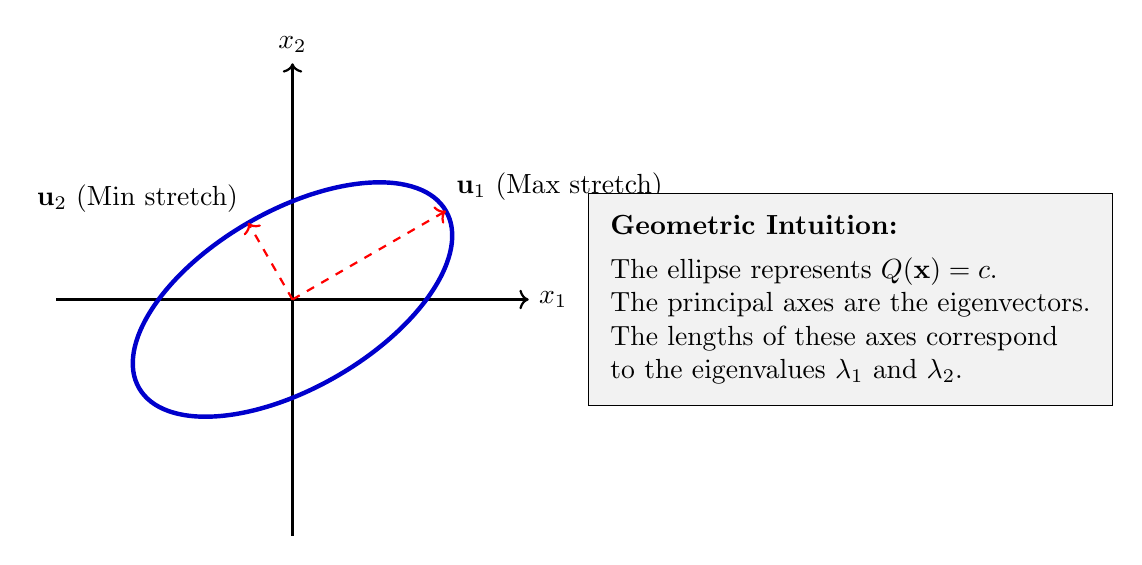
\begin{tikzpicture}[scale=1.5]
    % Background fill for stability
    \fill[white] (-2,-2) rectangle (2,2);
    
    % Grid and Axes
    \draw[thick, ->] (-2,0) -- (2,0) node[right] {$x_1$};
    \draw[thick, ->] (0,-2) -- (0,2) node[above] {$x_2$};
    
    % Ellipse (Quadratic Form Contour)
    \draw[ultra thick, blue!80!black, rotate=30] (0,0) ellipse (1.5cm and 0.75cm);
    
    % Principal Axes (Eigenvectors)
    \draw[thick, red, dashed, ->] (0,0) -- (30:1.5) node[above right, black] {$\mathbf{u}_1$ (Max stretch)};
    \draw[thick, red, dashed, ->] (0,0) -- (120:0.75) node[above left, black] {$\mathbf{u}_2$ (Min stretch)};
    
    % Annotation Node
    \node[align=left, anchor=west, inner sep=8pt, draw, fill=gray!10] at (2.5, 0) {
        \textbf{Geometric Intuition:}\\[4pt]
        The ellipse represents $Q(\mathbf{x}) = c$.\\
        The principal axes are the eigenvectors.\\
        The lengths of these axes correspond\\
        to the eigenvalues $\lambda_1$ and $\lambda_2$.
    };
\end{tikzpicture}
\end{center}

\subsection{Forward and Backward Links}
\textbf{Backward Links:} This topic relies heavily on the Spectral Theorem from earlier in linear algebra, which guarantees that symmetric matrices can be orthogonally diagonalized. It also connects to Multivariable Calculus, specifically Lagrange Multipliers. In fact, maximizing $\mathbf{x}^T A \mathbf{x}$ subject to $\mathbf{x}^T\mathbf{x} = 1$ using Lagrange Multipliers yields the equation $\nabla(\mathbf{x}^T A \mathbf{x}) = \lambda \nabla(\mathbf{x}^T\mathbf{x}) \implies 2A\mathbf{x} = 2\lambda\mathbf{x} \implies A\mathbf{x} = \lambda\mathbf{x}$. Thus, the eigenvalue problem is literally the Lagrange Multiplier problem in matrix form!

\textbf{Forward Links:} This is the direct foundation for the \textbf{Singular Value Decomposition (SVD)}, which is introduced in the very next section of your textbook. SVD extends this concept to non-square matrices by optimizing $\|A\mathbf{x}\|^2 = \mathbf{x}^T (A^T A) \mathbf{x}$. It is also the mathematical bedrock for Principal Component Analysis (PCA) in statistics.

\newpage

\section{Part 6: Abstract Real-World Modeling (AI, ML, \& Quant Finance)}

\subsection{Concrete Scenarios}
1. \textbf{Principal Component Analysis (PCA) in Machine Learning:} In high-dimensional datasets (like images or genomic data), we want to project the data onto a lower-dimensional subspace that captures the most variance. This is formulated as maximizing the quadratic form $\mathbf{w}^T \Sigma \mathbf{w}$ (where $\Sigma$ is the covariance matrix) subject to $\|\mathbf{w}\| = 1$. The solution is the dominant eigenvector of $\Sigma$.
2. \textbf{Portfolio Optimization in Quantitative Finance:} Modern Portfolio Theory (Markowitz) seeks to minimize the variance (risk) of a portfolio for a given expected return. The risk is a quadratic form $\mathbf{w}^T \Sigma \mathbf{w}$, where $\mathbf{w}$ are the asset weights and $\Sigma$ is the covariance matrix of asset returns.

\subsection{Model Problem Setup: Markowitz Portfolio Optimization}
Let us build a rigorous mathematical model for the Quantitative Finance scenario.
Define a state space of $n$ risky assets. Let $\mathbf{R} = [R_1, R_2, \dots, R_n]^T$ be the random vector of asset returns with expected value $\E[\mathbf{R}] = \boldsymbol{\mu}$ and positive-definite covariance matrix $\Sigma = \E[(\mathbf{R} - \boldsymbol{\mu})(\mathbf{R} - \boldsymbol{\mu})^T]$.

An investor wants to allocate capital across these assets. Let $\mathbf{w} \in \R^n$ be the weight vector, subject to the budget constraint $\mathbf{w}^T \mathbf{1} = 1$ (fully invested). The portfolio return is the random variable $R_p = \mathbf{w}^T \mathbf{R}$.
The expected return is $\mu_p = \mathbf{w}^T \boldsymbol{\mu}$, and the portfolio variance (risk) is $\sigma_p^2 = \mathbf{w}^T \Sigma \mathbf{w}$.

The investor seeks to minimize risk subject to achieving a target expected return $\mu_0$. This is a constrained optimization problem of a quadratic form:
\[ \min_{\mathbf{w}} \quad \frac{1}{2} \mathbf{w}^T \Sigma \mathbf{w} \]
\[ \text{subject to} \quad \mathbf{w}^T \mathbf{1} = 1 \quad \text{and} \quad \mathbf{w}^T \boldsymbol{\mu} = \mu_0 \]
Using Lagrange multipliers $\lambda_1, \lambda_2$, the Lagrangian is:
\[ \mathcal{L}(\mathbf{w}, \lambda_1, \lambda_2) = \frac{1}{2} \mathbf{w}^T \Sigma \mathbf{w} - \lambda_1 (\mathbf{w}^T \mathbf{1} - 1) - \lambda_2 (\mathbf{w}^T \boldsymbol{\mu} - \mu_0) \]
Taking the gradient with respect to $\mathbf{w}$ and setting it to zero yields:
\[ \nabla_{\mathbf{w}} \mathcal{L} = \Sigma \mathbf{w} - \lambda_1 \mathbf{1} - \lambda_2 \boldsymbol{\mu} = \mathbf{0} \implies \mathbf{w} = \Sigma^{-1} (\lambda_1 \mathbf{1} + \lambda_2 \boldsymbol{\mu}) \]
This shows that the optimal portfolio weights are a linear combination of the vectors $\Sigma^{-1}\mathbf{1}$ and $\Sigma^{-1}\boldsymbol{\mu}$, deeply linking matrix inversion and quadratic optimization to financial risk management.

\newpage

\section{Part 7: Common Variations and Untested Concepts}

\subsection{Variation: Non-Unit Sphere Constraints (Generalized Eigenvalue Problem)}
The homework exclusively tested constraints of the form $\mathbf{x}^T\mathbf{x} = 1$ (a standard unit sphere). A common advanced variation is optimizing a quadratic form subject to an elliptical constraint, such as $\mathbf{x}^T B \mathbf{x} = 1$, where $B$ is a symmetric positive-definite matrix.

This leads to the \textbf{Generalized Eigenvalue Problem}. Using Lagrange multipliers to maximize $\mathbf{x}^T A \mathbf{x}$ subject to $\mathbf{x}^T B \mathbf{x} = 1$, we get:
\[ \nabla(\mathbf{x}^T A \mathbf{x}) = \lambda \nabla(\mathbf{x}^T B \mathbf{x}) \implies 2A\mathbf{x} = 2\lambda B\mathbf{x} \implies A\mathbf{x} = \lambda B\mathbf{x} \]
The maximum value is still the largest generalized eigenvalue $\lambda$, but finding it requires solving $\det(A - \lambda B) = 0$.

\textbf{Worked Example:}
Maximize $Q(\mathbf{x}) = 3x_1^2 + 2x_2^2$ subject to the constraint $2x_1^2 + x_2^2 = 1$.
\textit{Solution:}
Here, $A = \begin{bmatrix} 3 & 0 \\ 0 & 2 \end{bmatrix}$ and $B = \begin{bmatrix} 2 & 0 \\ 0 & 1 \end{bmatrix}$.
We solve $\det(A - \lambda B) = 0$:
\[ \det \begin{bmatrix} 3 - 2\lambda & 0 \\ 0 & 2 - \lambda \end{bmatrix} = (3 - 2\lambda)(2 - \lambda) = 0 \]
The generalized eigenvalues are $\lambda = 1.5$ and $\lambda = 2$.
The maximum value is the largest eigenvalue, which is $2$. This occurs when $3 - 2\lambda \neq 0$, meaning the eigenvector corresponds to the second coordinate. Setting $x_1 = 0$, the constraint $2(0)^2 + x_2^2 = 1 \implies x_2 = \pm 1$. Thus, the maximum is $2$, attained at $(0, 1)$.

\newpage

\section{Part 8: Advanced Diagnostic Testing: "Find the Flaw"}

Below are 5 problems with step-by-step solutions that contain a single, critical flaw. Your task as the grader is to identify the error, explain why it is wrong, and provide the correct final answer.

\vspace{1em}
\textbf{Problem 1:} Find the maximum value of $Q(\mathbf{x}) = 4x_1^2 + 6x_1x_2 + 4x_2^2$ subject to $x_1^2 + x_2^2 = 1$.
\textit{Flawed Solution:}
1. The matrix for the quadratic form is $A = \begin{bmatrix} 4 & 6 \\ 6 & 4 \end{bmatrix}$.
2. The characteristic equation is $(4-\lambda)^2 - 36 = 0 \implies 4-\lambda = \pm 6$.
3. The eigenvalues are $\lambda = 10$ and $\lambda = -2$.
4. The maximum value is 10.
\textit{Find the Flaw:} \hrulefill \\
\textit{Correction:} \hrulefill

\vspace{1em}
\textbf{Problem 2:} Find a unit vector that maximizes $Q(\mathbf{x}) = 2x_1^2 + 2x_2^2$ subject to $x_1^2 + x_2^2 = 1$.
\textit{Flawed Solution:}
1. The matrix is $A = \begin{bmatrix} 2 & 0 \\ 0 & 2 \end{bmatrix}$.
2. The eigenvalue is $\lambda = 2$ (multiplicity 2).
3. We solve $(A - 2I)\mathbf{x} = \mathbf{0}$, which gives the zero matrix. Thus, any vector is an eigenvector.
4. I choose the vector $\mathbf{x} = \begin{bmatrix} 1 \\ 1 \end{bmatrix}$.
5. The maximum is attained at $\mathbf{x} = \begin{bmatrix} 1 \\ 1 \end{bmatrix}$.
\textit{Find the Flaw:} \hrulefill \\
\textit{Correction:} \hrulefill

\vspace{1em}
\textbf{Problem 3:} Find the maximum value of $Q(\mathbf{x}) = -3x_1^2 - 8x_2^2$ subject to $x_1^2 + x_2^2 = 1$.
\textit{Flawed Solution:}
1. The matrix is $A = \begin{bmatrix} -3 & 0 \\ 0 & -8 \end{bmatrix}$.
2. The eigenvalues are $-3$ and $-8$.
3. Since we want the maximum value, we look for the eigenvalue with the largest magnitude.
4. $|-8| > |-3|$, so the maximum value is $-8$.
\textit{Find the Flaw:} \hrulefill \\
\textit{Correction:} \hrulefill

\vspace{1em}
\textbf{Problem 4:} Let $A = \begin{bmatrix} 5 & 2 \\ 2 & 8 \end{bmatrix}$. Find the maximum of $\mathbf{x}^T A \mathbf{x}$ subject to $\mathbf{x}^T\mathbf{x} = 1$ and $\mathbf{x}^T\mathbf{u}_1 = 0$, where $\mathbf{u}_1$ is the eigenvector for the largest eigenvalue.
\textit{Flawed Solution:}
1. The characteristic equation is $(5-\lambda)(8-\lambda) - 4 = \lambda^2 - 13\lambda + 36 = 0$.
2. The eigenvalues are $\lambda = 9$ and $\lambda = 4$.
3. The largest eigenvalue is 9.
4. The constraint $\mathbf{x}^T\mathbf{u}_1 = 0$ means we must find the minimum value of the quadratic form.
5. Therefore, the answer is 4.
\textit{Find the Flaw:} \hrulefill \\
\textit{Correction:} \hrulefill

\vspace{1em}
\textbf{Problem 5:} Find the change of variable $\mathbf{x} = P\mathbf{y}$ that diagonalizes $Q(\mathbf{x}) = 2x_1^2 - 4x_1x_2 + 5x_2^2$.
\textit{Flawed Solution:}
1. $A = \begin{bmatrix} 2 & -2 \\ -2 & 5 \end{bmatrix}$.
2. Eigenvalues are $\lambda_1 = 6, \lambda_2 = 1$.
3. Eigenvector for $\lambda=6$ is $\mathbf{v}_1 = \begin{bmatrix} -1 \\ 2 \end{bmatrix}$. Eigenvector for $\lambda=1$ is $\mathbf{v}_2 = \begin{bmatrix} 2 \\ 1 \end{bmatrix}$.
4. We construct $P = \begin{bmatrix} -1 & 2 \\ 2 & 1 \end{bmatrix}$.
5. The change of variable is $\mathbf{x} = \begin{bmatrix} -1 & 2 \\ 2 & 1 \end{bmatrix} \mathbf{y}$.
\textit{Find the Flaw:} \hrulefill \\
\textit{Correction:} \hrulefill

\end{document}